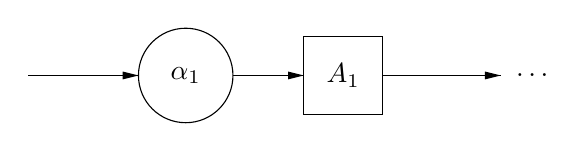
\begin{tikzpicture}[scale=0.2]
\tikzstyle{every node}+=[inner sep=0pt]
\draw [black] (-20,0) -- (-13,0);
\fill [black] (-13,0) -- (-14,-.25) -- (-14,+.25);

\draw [black] (-10,0) circle (3);
\draw [black] (-10,0) node {$\alpha_1$};

\draw [black] (-7,0) -- (-2.5,0);
\fill [black] (-2.5,0) -- (-3.5,-.25) -- (-3.5,+.25);

\draw [black] (-2.5,-2.5) -- (-2.5,+2.5) -- (+2.5,+2.5) -- (+2.5,-2.5) -- cycle;
\draw [black] (0,0) node {$A_1$};

\draw [black] (+2.5,0) -- (+10,0);
\fill [black] (+10,0) -- (+9,-.25) -- (+9,+.25);

\draw [black] (+12,0) node {$\ldots$};
\end{tikzpicture}
